\documentclass[a4paper,11pt]{article}

%%%%%%%%%%%%%%%%%%%%%%%%%%%%%%%%%
%            ATENÇÃO            %
% NÃO ALTERE AS LINHAS A SEGUIR %
%%%%%%%%%%%%%%%%%%%%%%%%%%%%%%%%%

\usepackage[brazil]{babel}
\usepackage{float,graphicx,graphics,amssymb,amsfonts,newlfont,indentfirst}
\usepackage[centertags]{amsmath}
\usepackage{fancyhdr}
\usepackage{ragged2e}
\usepackage{geometry}
\geometry{top=0cm,bottom=2cm,left=3cm,right=2cm}
\usepackage[normalem]{ulem}
\pagestyle{fancy}
\usepackage{url}
\usepackage{color}
\usepackage[font+=small,leftmargin=4cm,rightmargin=0cm,indentfirst=false]{quoting}
%\fancyfoot{} %retira número das páginas do rodapé
\renewcommand{\rmdefault}{ptm}
\renewcommand{\sfdefault}{ptm}
\renewcommand{\ttdefault}{ptm}

\lhead{ERMAC, Volta Redonda -- RJ, 2023}

\fancypagestyle{capa}{%
	\fancyhead{}%
	\rhead{\textit{Trabalho apresentado no ERMAC, Volta Redonda -- RJ, 2023.}%
	\vspace*{11pt}}%
}

\usepackage{mathptmx} % Fonte Times em fórmulas

\headheight 10mm
\oddsidemargin 2.0mm
\evensidemargin 2.0mm
\topmargin -10mm
\textheight 240mm
\textwidth 160mm
\headsep 5mm
\parindent 1mm


%%%%%%%%%%%%%%%%%%%%%%%%%%%%%
% MODIFIQUE DAQUI EM DIANTE %
%%%%%%%%%%%%%%%%%%%%%%%%%%%%%

% pacotes adicionais
%\usepackage{algorithm}
\usepackage[pdftex]{hyperref} %permite resaltar texto
\hypersetup{colorlinks,citecolor=black,filecolor=black,linkcolor=black,urlcolor=black} %setup de hyperref
\bibliographystyle{unsrt}
\bibliographystyle{abntex2-alf}

\begin{document}

\centering{{\Large{\bf Herramienta para la simulacion del crecimiento de tumores en diversas regiones del cuerpo humano en 3 dimensiones.}}

\begin{flushright}{\it
\vspace*{5mm}
Carlos Carret Miranda\\
Universidad de la Habana\\
carlos.carret@estudiantes.matcom.uh.cu

\vspace*{5mm}
\underline{ Reinaldo Rodríguez Ramos}\\
Departamento de Matem\'aticas, Facultad de Matem\'aticas y Computaci\'on, Universidad de La Habana, Cuba y PPG-MCCT, Universidade Federal Fluminense, Volta Redonda, Rio de Janeiro, Brazil.\\
reinaldo@matcom.uh.cu and reinaldorr@id.uff.br

\vspace*{5mm}
Panters Rodríguez Bermúdez\\
Departamento de Ciências Exatas, Universidade Federal Fluminense, Volta Redonda, Rio de Janeiro, Brazil\\
pantersrb@id.uff.br

% se necessário, adicione mais autores como nos blocos acima
}\end{flushright}


\setcounter{equation}{0} % NÃO modifique esta linha


\thispagestyle{capa}
\justifying{
{\noindent \bf Resumo: }{\small{%
	%RESUMO 
 Cancer is a disease characterized by the uncontrolled growth of abnormal cells in the body. It is a complex and multifaceted disease that has challenged researchers and doctors for decades. The ability to visualize and understand tumor growth can provide valuable insights into how cancer develops and spreads, leading to significant improvements in cancer diagnosis, treatment, and prevention. The three-dimensional tumor growth simulation tool that is being developed is an important step in this direction. It allows for detailed visualization of tumor growth in different parts of the human body, which can provide valuable insights into how cancer develops and spreads. Additionally, the ability of this tool to simulate tumor growth in different parts of the body means that it can be used to study a wide range of cancer types. This tool utilizes a cellular automaton and a small-world network to create connections between cells, allowing for a more accurate representation of organ and tumor structures. Furthermore, it allows for the loading of configurations and parameters from external files, providing great flexibility to the tool and allowing for customization of the simulation to the specific needs of each case. For 3D rendering, the Marching Cubes technique is used, which enables detailed and accurate three-dimensional representation of tumors.
}}

\vskip 0.2cm  % NÃO modifique esta linha


{\small{ %PALAVRAS-CHAVE
\noindent{\bf{Palavras-chave:}} Cellular Automaton, Marching Cubes, 3D, cancer, tumor
}}
}

%%%%%%%%%%%%%%%%%%%%%%%%%%%%%
%%%%%%%%%%%%%%%%%%%%%%%%%%%%%

\section*{Introdução}

The challenge of representing biological phenomena mathematically, physically, and computationally requires interdisciplinary synergy among experts in these fields. This collaboration enriches the traditional experimental method used in biological sciences by implementing mathematical models, which serve as tools to formulate and test hypotheses, guide experimental research, and refine the model based on the obtained results.~\cite{Darien}

Cancer is a disease that affects a large number of living organisms and is characterized by the presence of a group of abnormal cells that grow uncontrollably, disregarding the normal rules of cell division. It particularly affects humans, where its occurrence and development pose a threat to life. The malignancy of cancer varies and depends on factors such as the growth rate of cancer cells, their ability to spread to other tissues, and the possibility of recurrence after surgical removal.

The purpose of this type of research is to achieve a deeper understanding of biological processes through an iterative cycle of theory and experimentation. Additionally, mathematical models can be used to assist in the conception and design of therapeutic strategies, providing a more precise and personalized insight into the treatment of each patient.

In the case of this project, a cellular automaton and a small-world network are used to model the interactions between cells, providing a more accurate representation of tumor growth. The parameters and configurations can be loaded from external files, offering great flexibility in adapting the simulation to the specific needs of each case.

The technique of Marching Cubes~\cite{paper de Marching Cubes} is used for 3D rendering, providing a detailed and precise visualization of tumors. This visualization can provide valuable insight into how cancer develops and spreads, which can be essential for the development of effective therapies and treatments. By visualizing tumor growth in three dimensions, doctors and scientists can gain a better understanding of tumor evolution and how it may affect surrounding tissues. This information can be crucial for the development of effective therapies and treatments for cancer.


\section*{Submissão}

\textbf{Cellular Automaton}

In this section, the cellular automaton model presented in this work is conceived. It begins by formally defining a cellular automaton~\cite{5}.

A cellular automaton is a tuple $(\mathcal{L}; \mathcal{N}; \mathcal{E}; \mathcal{R})$ composed of the following representative elements:
\begin{itemize}
\item [$\mathcal{L}$:] t is a potentially infinite set of cells.
\item [$\mathcal{N}$:] $\mathcal{L} \times \mathcal{L} \rightarrow \lbrace 0,1 \rbrace$ is a neighborhood function, which can be seen as a relation, usually reflexive and symmetric, between cells. This function shows which pairs of cells are neighbors, that is, the geometry of the cellular organization.
\item [$\mathcal{E}$:] It is a set of states. Each cell in the set $\mathcal{L}$ is assigned an associated state at each time step.
\item [$\mathcal{R}$:] $\mathcal{E}^{|\mathcal{N}(v)|} \rightarrow \mathcal{E}$ is a locally defined transition function. This function is the core of the dynamics of a cellular automaton and is commonly expressed through rules that define the state of the cell in the next time step based on the state of the neighboring cells. The set containing the state of the neighboring cells is obtained through the function $\mathcal{N}(v)$, wich is defined below ~\ref{1}.
\end{itemize}

The sets $A^n(G)$ and $A^d(G)$ group the edges of the graph that correspond to immediate and distant connections, respectively. These sets have the following properties:
\begin{subequations}
\begin{equation}
A^n(G) \cup A^d(G) = A(G),
\end{equation}
\begin{equation}
A^n(G) \cap A^d(G) = \emptyset.
\end{equation}
\end{subequations}
These properties indicate that the subsets of edges $A^n(G)$ and $A^d(G)$ form a partition of the set of edges $A(G)$

Based on the sets of vertices $V(G)$ and edges $A(G)$, the representative elements $\mathcal{L}$ and $\mathcal{N}$ of the cellular automaton model are defined as follows:

The set of cells $\mathcal{L}$ is defined based on the set of vertices of the graph $V(G)$ as shown below:
\begin{align}
\boxed{\mathcal{L} = V(G)}~. \label{eq-L}
\end{align}

The neighborhood function $\mathcal{N}$ s defined based on the set of edges of the graph $A(G)$ as shown below:
\begin{subequations}
\begin{equation}
\boxed{\mathcal{N} : V(G) \times V(G) \rightarrow \lbrace 0,1 \rbrace}~, \label{eq-N}
\end{equation}
\begin{equation}
\boxed{\mathcal{N}(v,w) = \left\lbrace
	\begin{array}{lr}
		0& \textit{si } \lbrace v,w \rbrace \notin A(G)\\
		1& \textit{si } \lbrace v,w \rbrace \in A(G)
	\end{array}
\right.}~, \label{eq-N-2}
\end{equation}
\end{subequations}
In other words, the vertices $v \in V(G)$ and $w \in V(G)$  are neighbors in the cellular automaton if there exists an edge in $G$ that connects them.

The neighborhood of the vertex $v \in V(G)$ is defined based on the neighborhood function $\mathcal{N}(v,w)$   as the set of vertices $\mathcal{N}(v)$  that have edges with the vertex $v$:
\begin{align} 
\mathcal{N}(v) = \lbrace w~|~\mathcal{N}(v,w)=1 \rbrace. \label{eq-neighbourhood}
\end{align}
\\
\textbf{Set of cells: Watts-Strogatz model}

In the presented study, a soft tissue is defined as a set of cells that exhibit two types of connections: between nearby neighboring cells and between distant cells. To represent these types of connections, a cellular automaton model based on a graph network is used. In their work[31], Duncan J. Watts and Steven H. Strogatz showed that there are many biological, technological, and social networks that lie between regular and random networks, which have traditionally been used to model different types of dynamic systems.

Let $v$ be a vertex of the graph that has $k_v$ edges connecting it to $k_v$ vertices. The value between the actual number of edges $K_v$ that exist between these $k_v$ vertices and the maximum number of possible edges\footnote{El n\'umero m\'aximo de aristas posibles se alcanza cuando los $k_v$ vecinos del v\'ertice $v$ pertenecen a un clique. Un clique en un grafo no dirigido es un conjunto de v\'ertices tal que para todo par de v\'ertices, existe una arista que los conecta.} $k_v(k_v-1)/2$ e is the clustering coefficient of vertex $v$ and is determined as~\cite{Darien Tesis}:
\begin{align}
C_v = \displaystyle\frac{2K_v}{k_v(k_v-1)}. \label{eq-clustering}
\end{align}

The global clustering coefficient of the graph $C_G$ is the average of all individual clustering coefficients $C_v$, that is~\cite{Darien Tesis}:
\begin{align}
C_G = \displaystyle\frac{1}{|V(G)|}\sum _{v=1} ^{|V(G)|} C_v. \label{eq-global-clustering}
\end{align}

The average path length is the mean of the distances between every pair of vertices belonging to the graph and is denoted as $\ell_G$. Due to the existence of numerous distant connections through the circulatory system, the average path length in the network of cells is relatively small.

Therefore, it is hypothesized that a living tissue possesses a high clustering coefficient and a small average path length. These characteristics are characteristic of small-world networks, and they are used to represent living tissue. To generate small-world networks with these characteristics, the Watts and Strogatz model is used~\cite{31}. This model starts with a graph with $q$ vertices, each connected to $k$ immediate neighbors, and then randomly rewires each edge of the graph with a probability $p$, introducing edges that connect distant vertices.\\
\\
\textbf{Marching Cubes}

La técnica de Marching Cubes es un algoritmo de gráficos por computadora que se usa para extraer una malla poligonal de una isosuperficie de un campo escalar discreto tridimensional, como lo son los datos de imágenes de tomografías computarizadas y resonancias magnéticas ~\cite{7}. En el contexto de nuestro proyecto, se utiliza para la representación tridimensional de los tumores, proporcionando una visualización detallada y precisa.

Este algoritmo trabaja procesando las celdas de los datos de volumen (también conocidas como vóxeles), verificando la intersección entre sus respectivas aristas y la isosuperficie. Los valores de cada vértice de las celdas se comparan con un valor isosuperficial dado, y estos vértices se clasifican como "dentro" o "fuera" de la isosuperficie. Una vez definido el tipo de intersección, se realiza una aproximación de la isosuperficie contenida en la celda construyendo triángulos ~\cite{6}.

La visualización resultante puede proporcionar una comprensión valiosa de cómo se desarrolla y se propaga el cáncer. Al visualizar el crecimiento del tumor en tres dimensiones, los médicos y científicos pueden obtener una mejor comprensión de la evolución del tumor y cómo puede afectar a los tejidos circundantes. Esta información puede ser esencial para el desarrollo de terapias y tratamientos efectivos para el cáncer 

En resumen, la técnica de Marching Cubes es una herramienta potente para la visualización tridimensional de datos médicos. En el contexto de la investigación del cáncer, puede proporcionar una representación detallada y precisa del crecimiento de los tumores, lo que puede contribuir significativamente a nuestra comprensión de esta enfermedad y al desarrollo de terapias y tratamientos efectivos.

Debido a que es muy costoso representar y aplicar el algoritmo de Marching Cubes para modelos tan realistas que contengan millones de celulas en este trabajo se lleva a cabo la implementacion de un escalado del modelo que permite reducir el tamano de las dimensiones de nuestro modelo original de automata celular. Para hacer semejante reduccion se procede de la siguiente forma:
\begin{itemize}
    \item Se agrupan las celulas por cuadrantes de dimension proporcionada por el usuario.
    \item Se buscan los estados de todas las celulas pertenecientes al cuadrante.
    \item El cuadrante adoptara el estado que mas se repita entre las celulas que pertenezcan al mismo.
    \item Luego de hacer esto por varios cuadrantes, cada uno reducira su tamano desde $(n x m x l)$ a $(1 x 1 x 1)$, siendo $n \leq S_{x} ,m \leq S_{y},l \leq S_{z}$. 
\end{itemize}
\\
\textbf{Configuraciones y Parametros de la simulacion}

Algunos de los parametros y configuraciones que se pueden modificar son:
\begin{itemize}
    \item S_{x}$ - Dimension del espacio declarado en el eje de las x.
    \item S_{y}$ - Dimension del espacio declarado en el eje de las y.
    \item S_{z}$ - Dimension del espacio declarado en el eje de las z.
    ~\cite{Tesis de Darien}
Los rangos de valores de las componentes espaciales de los vértices del grafo son los siguientes: $0 \leq x \leq S_{x}$, $0 \leq y \leq S_{y}$ y $0 \leq z \leq S_{z}$.

    \item p - Probabilidad de reconexi´on del modelo Watts-Strogatz.
    \item $P_0^a$, $P_0^v$ - Poblaciones iniciales de las etapas avascular y vascular respectivamente.
    ~\cite{Tesis de Darien}
    \item Parametros correspondientes a la cantidad de estados que pueden tener las celdas del automata y descripciones de los mismos.
    \item Parametros de posibles transiciones entre los estados del automata.
    \item Parametros de probabilidades para que ocurran las transiciones entre los estados.
    Al incluir parametros para el calculo de ciertas probabilidades, se puede tener en cuenta el calculo de la probabilidad de la interaccion de las celulas tumorales con el sistema inmune, como se hace en ~\cite{2}.
    \item Parametros correspondientes con la forma de los organos donde se desarrollara la simulacion.
    \item Parametros para describir el esquema de los organos donde se llevara a cabo la simulacion. De esta forma podemos tener en cuenta las caracteristicas de cada organo por separado y realizar una simulacion mas realista.
\end{itemize}

Existen muchos otros parametros que son configurables.\\

\section*{Seleção de trabalhos}

Os trabalhos submetidos, dentro do prazo estabelecido, serão enviados aos revisores do Comitê Científico. Com base nos pareceres do comitê, o trabalho poderá ser (1) aceito plenamente, (2) aceito sob a condição de que correções menores sejam feitas em curto prazo ou (3) rejeitado.


\section*{Citações}
Devem seguir as normas da ABNT NBR 10520. Nas citações, as chamadas pelo sobrenome do autor devem ser em letras maiúsculas e minúsculas e, quando estiverem entre parênteses, devem ser em letras maiúsculas.

Exemplos:

A ironia seria assim uma forma implícita de heterogeneidade mostrada, conforme a classificação proposta por Authier-Reiriz (1982).

\vskip 0.2cm
``Apesar das aparências, a desconstrução do logocentrismo não é uma psicanálise da filosofia [...]'' (DERRIDA, 1967, p. 293).

\vskip 0.2cm
a) As citações diretas, no texto, com mais de três linhas, devem ser destacadas com recuo de 4 cm da margem esquerda, espaço entre linhas simples e sem aspas, em fonte Times New Roman, tamanho 10.

\begin{quoting}
A teleconferência permite ao indivíduo participar de um encontro nacional ou regional sem a necessidade de deixar seu local de origem. Tipos comuns de teleconferência incluem o uso da televisão, telefone, e computador. Através de áudio-conferência, utilizando a companhia local de telefone, um sinal de áudio pode ser emitido em um salão de qualquer dimensão. (NICHOLS, 1993, p. 181).
\end{quoting}

\vskip 0.2cm
b) As citações diretas, no texto, de até três linhas, devem ser escritas entre ``aspas'' duplas e incorporadas ao texto.
Exemplos:
Barbour (1971, p. 35) descreve: ``O estudo da morfologia dos terrenos [...] ativos [...]''

\vskip 0.2cm
``Não se mova, faça de conta que está morta.'' (CLARAC; BONNIN, 1985, p. 72).

\vskip 0.2cm
Segundo Sá (1995, p. 27): ``[...] por meio da mesma `arte de conversação' que abrange tão extensa e significativa parte da nossa existência cotidiana [...]''

\vskip 0.2cm
c) Nas citações diretas, especificar no texto o ano de publicação e a(s) página(s) da fonte consultada. Estes dados devem ser colocados entre parênteses e separados por vírgula. Nas citações indiretas, a indicação da(s) página(s) consultada(s) é opcional, mas o ano de publicação da obra é obrigatório e deve estar entre parênteses.


\section*{Conclusões}

El crecimiento de un tumor puede ser visualizado en 3D utilizando la técnica de Marching Cubes. Se utiliza ampliamente para visualizaciones médicas, como imágenes de tomografía computarizada (TC) y resonancia magnética (RM). Además, el algoritmo de Marching Cubes puede reducir el tiempo de cálculo utilizado para el muestreo en la reconstrucción 3D. Sin embargo, uno de los problemas principales de Marching Cubes es la presencia de voxels no utilizados que pueden generarse durante el análisis de las coordenadas y los valores de intensidad de las imágenes 2D. Estos voxels no utilizados pueden afectar la suavidad de la superficie 3D ncbi.nlm.nih.gov.

\begin{figure}[h]
  \centering
  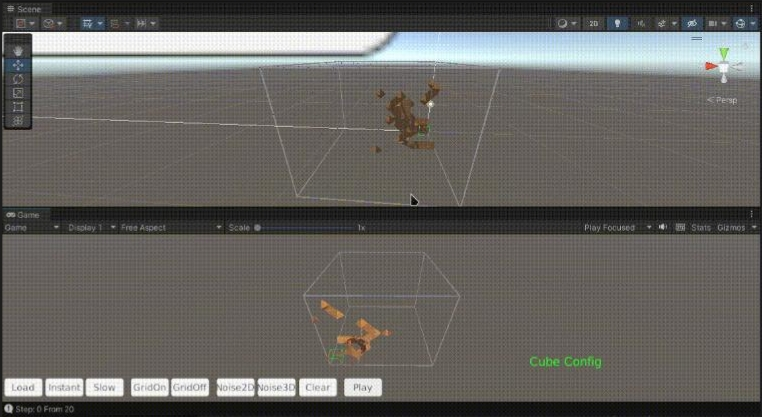
\includegraphics[width=0.9\textwidth]{tumor.jpg}
  \caption{Texto de la leyenda}
\end{figure}

La creación de una herramienta para simular el crecimiento de un tumor con un autómata celular en cualquier órgano del cuerpo humano es un avance significativo en el campo de la modelación y simulación de sistemas biológicos. Esta herramienta proporciona un enfoque innovador y flexible para estudiar el crecimiento de los tumores, lo cual tiene importantes implicaciones tanto en la investigación básica como en la clínica.

La capacidad de cargar configuraciones específicas y ajustar, agregar o eliminar parámetros que influyen en el realismo de la simulación permite adaptar el modelo a diferentes escenarios y condiciones. Esto hace que la herramienta sea altamente versátil y aplicable a una amplia gama de situaciones y tipos de tumores.

El uso de autómatas celulares para simular el crecimiento del tumor proporciona una representación detallada y dinámica del proceso. Los autómatas celulares son especialmente adecuados para este tipo de modelado, ya que permiten representar de forma precisa y realista la interacción entre las células y su entorno, así como los cambios que ocurren en el tiempo.

Finalmente, la visualización en 3D del crecimiento de un tumor utilizando la técnica de Marching Cubes puede proporcionar una herramienta valiosa para los profesionales de la salud para entender mejor la dinámica del crecimiento del tumor y desarrollar estrategias de tratamiento más efectivas.

\section*{Agradecimentos}

Os autores podem apresentar os agradecimentos a pessoas e instituições. Esta seção é OPCIONAL.



%%%%%%%%%%%%%%%%%%%%%%%%%%%%%
%%%%%%%%%%%%%%%%%%%%%%%%%%%%%

\section*{Referências}
{\color{red} A bibliografia deverá seguir o padrão da ABNT NBR 6023, separadas entre si por uma linha em branco, estar em \textbf{ordem alfabética pelo sobrenome do primeiro autor}, se necessário, usando-se, ainda, ordem cronológica, para trabalhos de um mesmo autor. Trabalhos dos mesmos autores, publicados no mesmo ano, devem ser listados utilizando-se a ordem alfabética do título do trabalho. Basicamente, as referências devem conter as iniciais dos nomes dos autores, sendo escrito, por extenso, apenas o último sobrenome. Seguem alguns exemplos:}


\begin{flushleft}

\begin{thebibliography}{99}
\bibitem{1} Guinot, V. Modelling using stochastic, finite state cellular automata: rule inference from continuum models. \textit{Applied Mathematical Modelling}, 26(6).

\vskip 0.2cm
\bibitem{2} Ruanxiaogang, H. A simple cellular automaton model for tumor-immunity system. In \textit{Robotics, Intelligent Systems and Signal Processing, 2003. Proceedings. 2003 IEEE International Conference on}, 2.

\vskip 0.2cm
\bibitem{3} Deutsch, A.; Maini, P.; Dormann, S. Cellular Automaton Modeling of Biological Pattern Formation: Characterization, Applications, and Analysis. \textit{Modeling and Simulation in Science, Engineering and Technology}. Birkhauser Boston, 2007.

\vskip 0.2cm
\bibitem{4} Kansal, A.; Torquato, S. Simulated brain tumor growth dynamics using a three-dimensional cellular automaton. \textit{Journal of Theoretical Biology}.

\vskip 0.2cm
\bibitem{5} Viera Barredo, D. Universidad de La Habana, Facultad de Matemática y Computación. Departamento de Matemática. Asesores: Reinaldo Rodríguez Ramos, Rubén Interián, Ariel Ramírez Torres, Rocío Rodríguez Sánchez. June, 2019.

\vskip 0.2cm
\bibitem{6} Cirne, M. A.; Pedrini, H. Marching cubes technique for volumetric visualization accelerated with graphics processing units. Journal of the Brazilian Computer Society, vol. 19, pages 223-233, 2013. Available at: https://journal-bcs.springeropen.com/articles/10.1007/s13173-012-0097-z. Accessed on [insert date].

\vskip 0.2cm
\bibitem{7} Lorensen, W. E.; Cline, H. E. Marching cubes: A high resolution 3D surface construction algorithm. ACM SIGGRAPH Computer Graphics, vol. 21, no. 4, pp. 163-169, Aug. 1987. Available at: https://en.wikipedia.org/wiki/Marching$\_$cubes. Accessed on [insert date].

\vskip 0.2cm
\bibitem{8} Visutsak, P. Marching Cubes and Histogram Pyramids for 3D Medical Visualization. Journal of Imaging, vol. 6, 2020. Available at: https://ncbi.nlm.nih.gov/pmc/articles/PMC8321043 and https://api.semanticscholar.org/CorpusID:225446991. Accessed on [insert date].

\vskip 0.2cm
\bibitem{31} Watts, D. J. \& Strogatz, S. H. Collective dynamics of small-world networks. \textit{Nature}, 393:440–442, 1998.


\end{thebibliography}

%Livro com até 3 autores:

\end{flushleft}

\end{document}
